\section{性能試験}
実際に製作した力覚センサに対する性能試験の結果について述べる. 
今回の試験は各起歪体ごとに行なった. 
ストッパ機構の働きを確認する試験は$F_z$成分の結果を示す. 

製作した力覚センサをFig.~\ref{fig:jissai}に示す.

\begin{figure}[h]
  \centering
  \subfloat[低剛性起歪体]{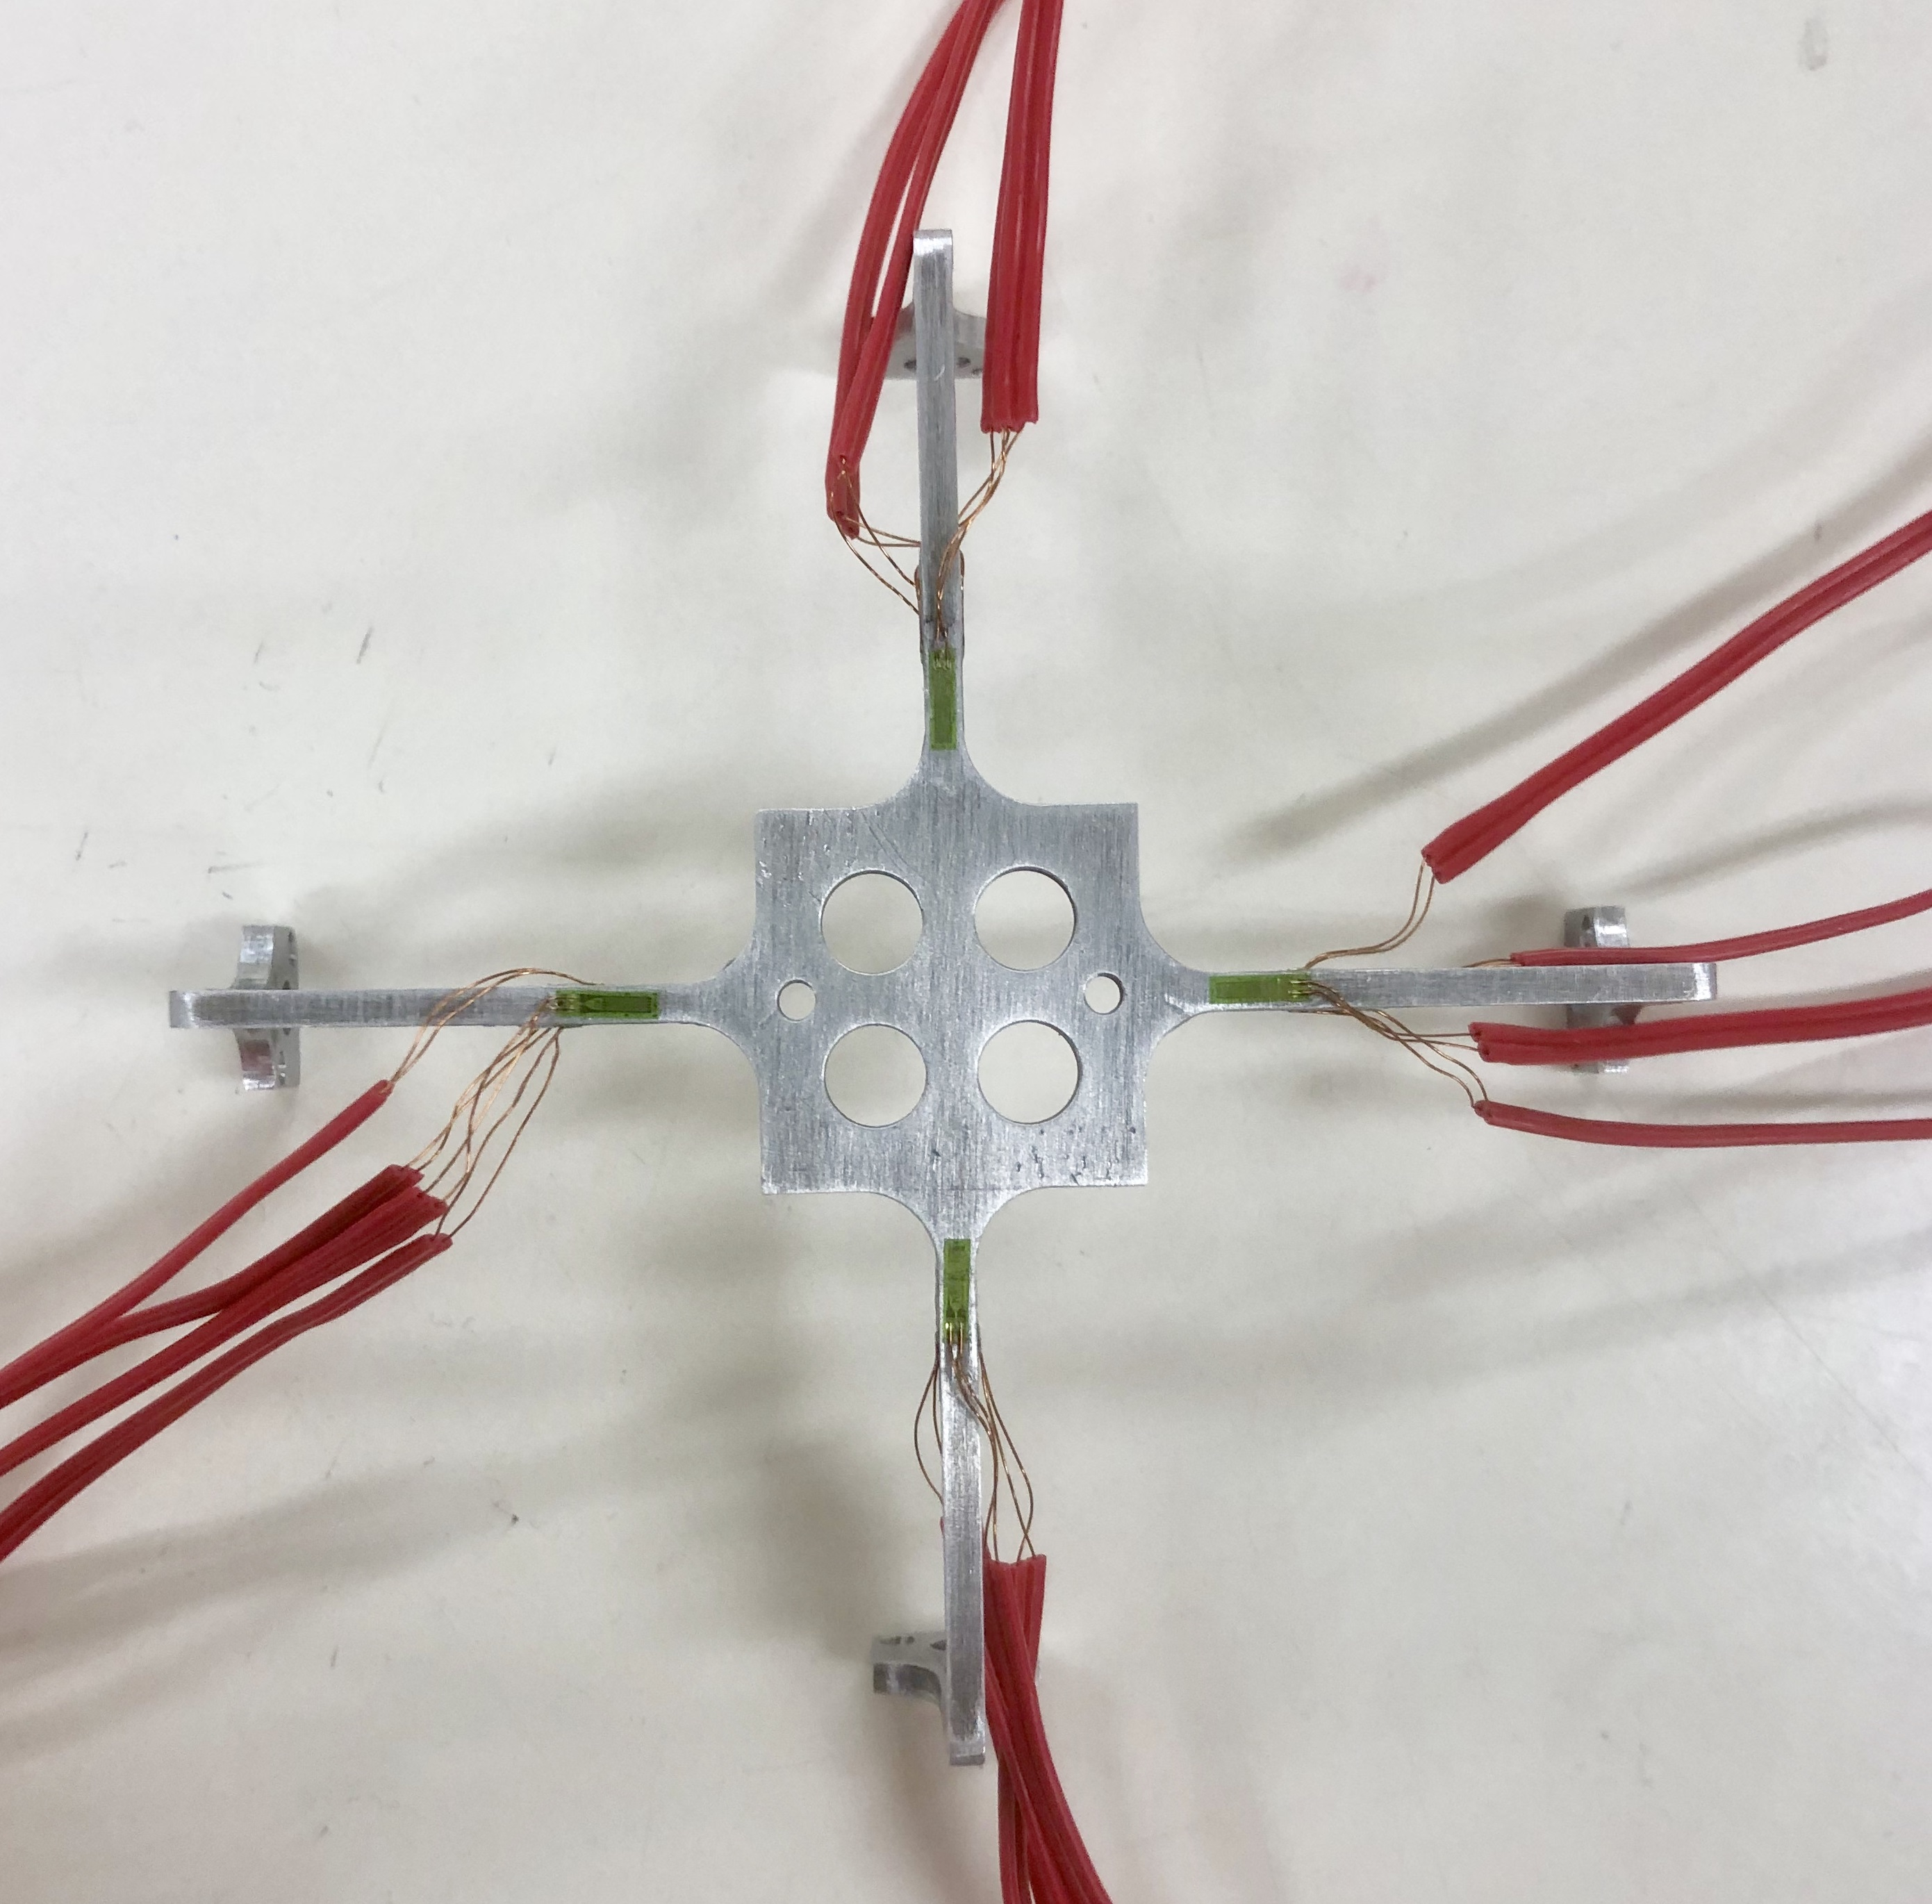
\includegraphics[width=4.2cm]{pic/real_L.jpg}}
  \subfloat[高剛性起歪体]{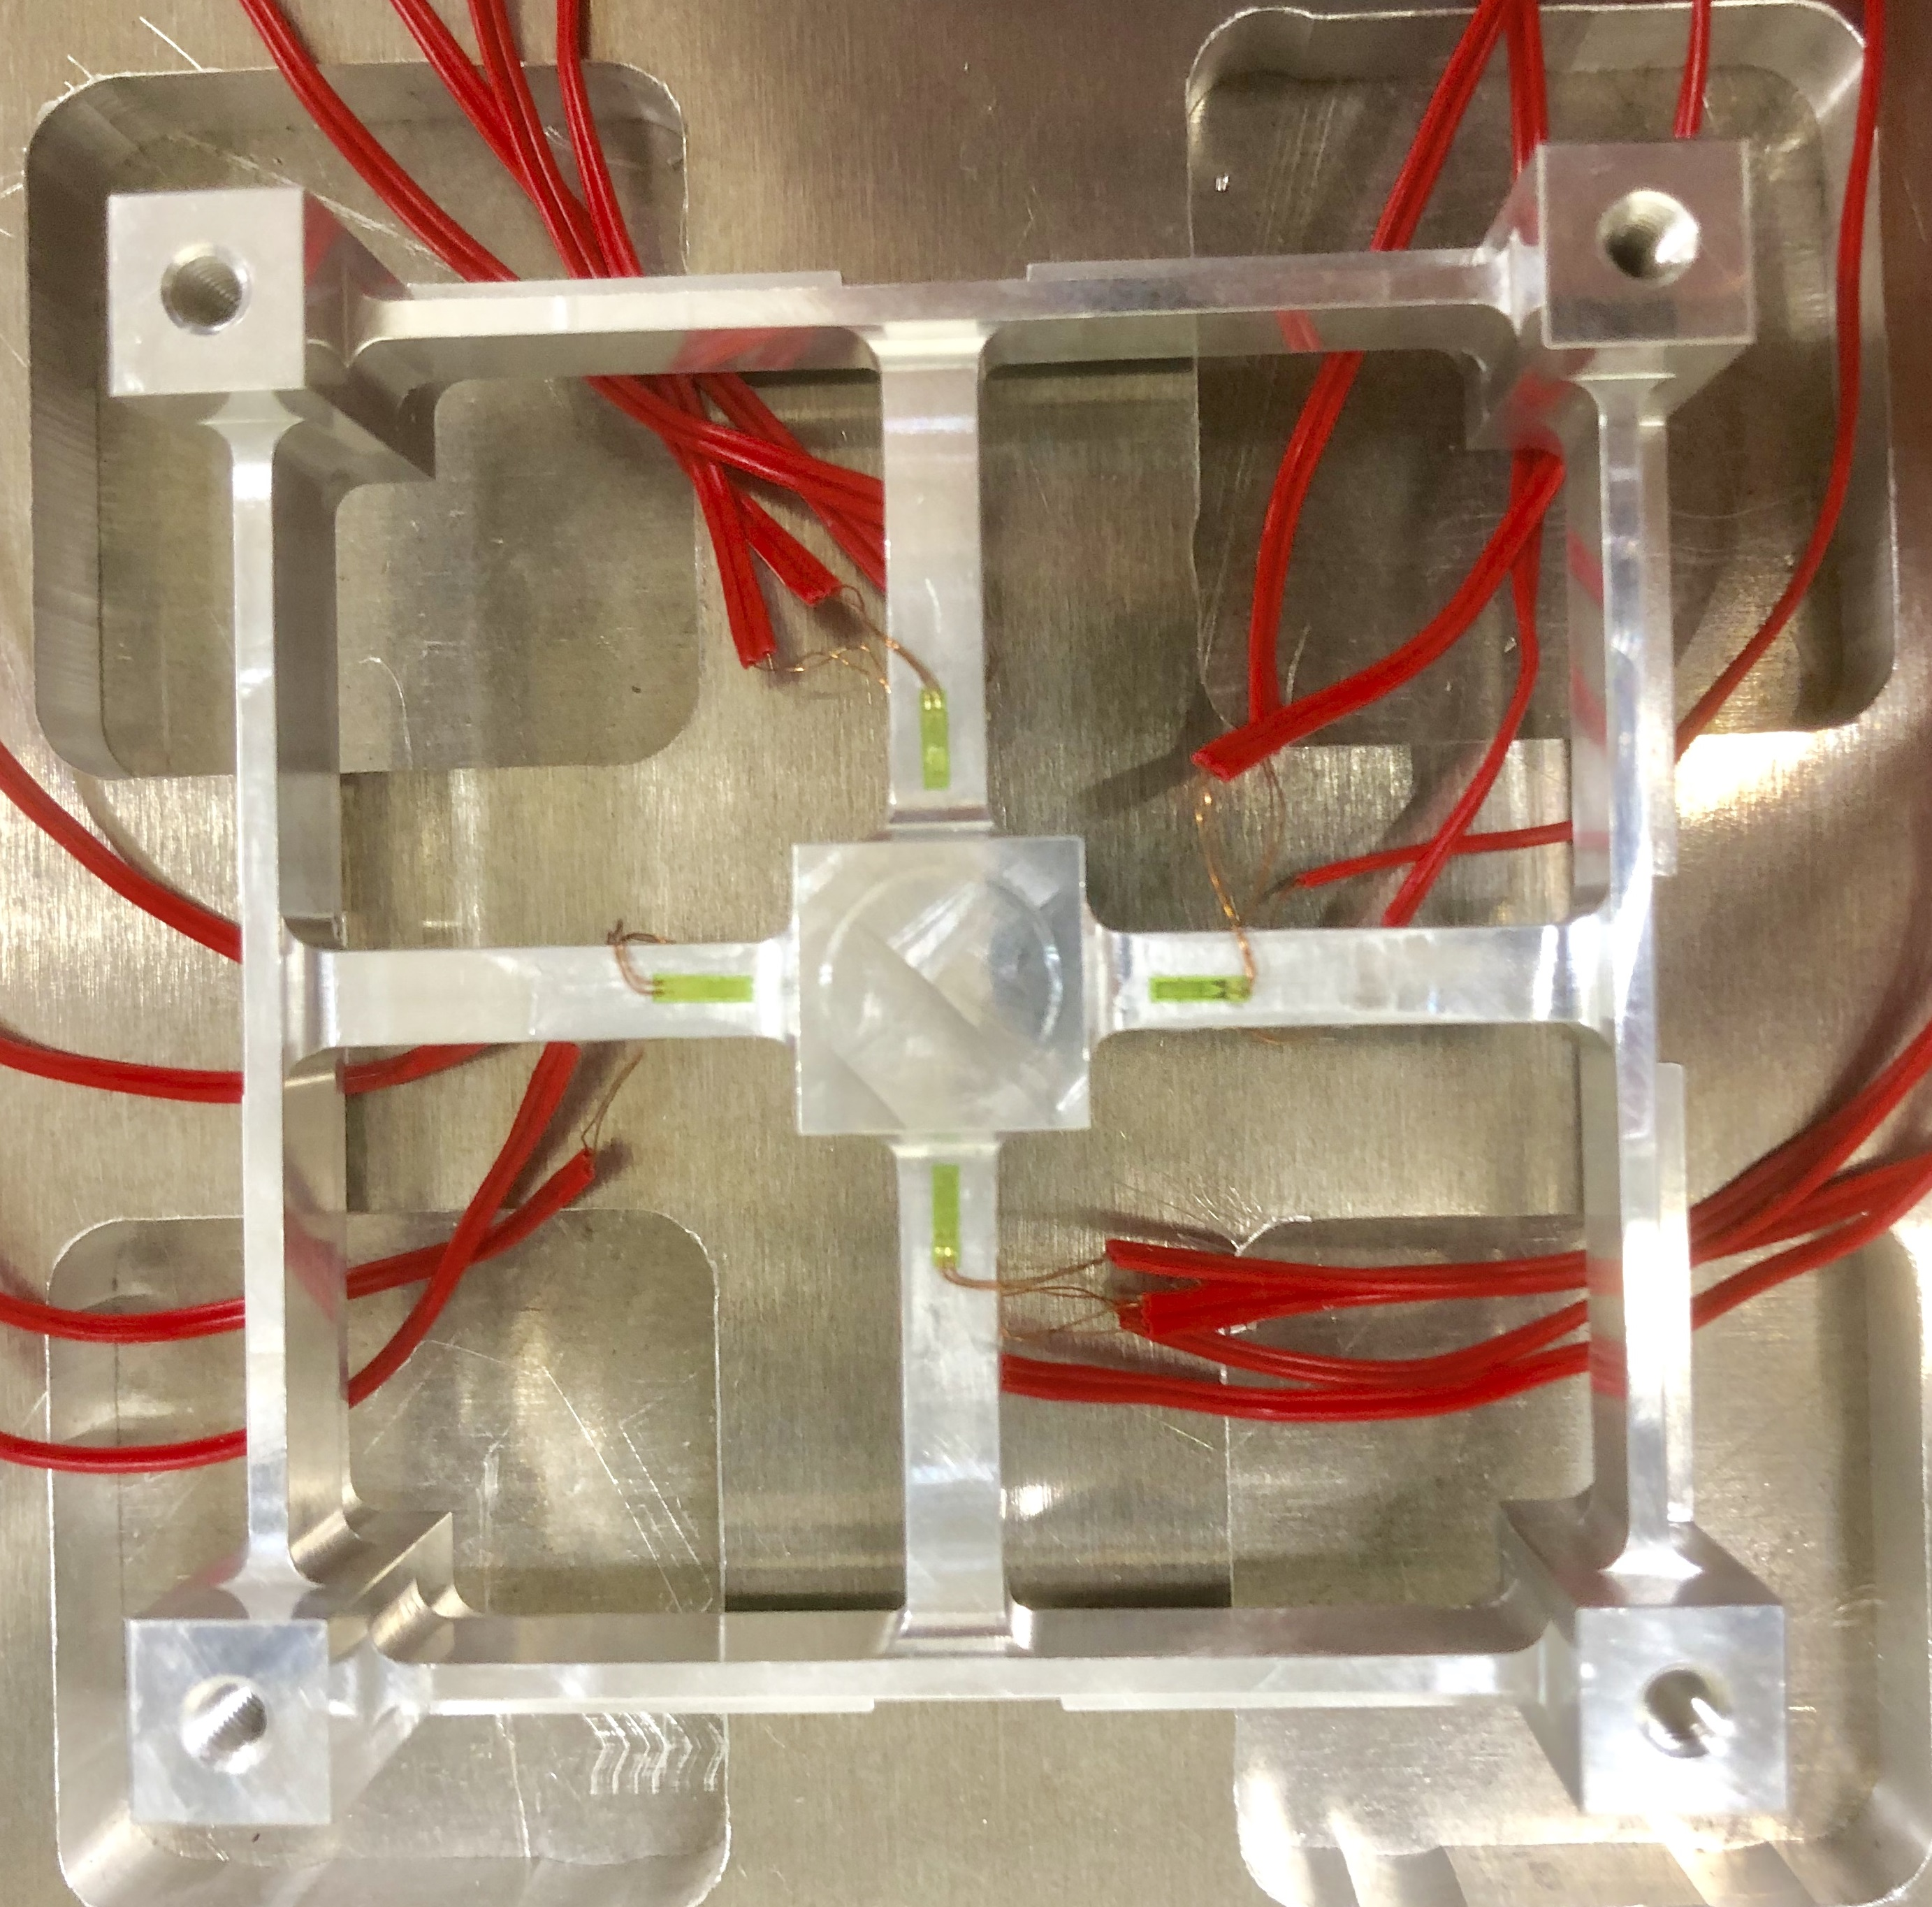
\includegraphics[width=4.2cm]{pic/real_H.jpg}}\\
  \caption[]{製作した小型HDR6軸力覚センサ}\label{fig:jissai}
\end{figure}

\subsection{非線形性・他軸干渉試験}
力覚センサは荷重-ひずみ変換行列を用いて印加荷重を算出する. 
印加された荷重に対する出力値の非線形性や, 
印加された荷重以外の成分の出力が応答する他軸干渉は
力覚センサの性能に関わる重要な指標である. 
 
\subsubsection*{低剛性起歪体}
任意に印加した荷重とひずみ出力の関係から式~\eqref{eq:c}をもとに
正負それぞれの荷重-ひずみ変換行列を算出した. 
\begin{eqnarray}
  \bm{C}^{-1}_{+low} = \left[
 \scalebox{0.7}{$\displaystyle
  \begin{array}{cccccc}
 13.4  &-9.8   &3.3  &-2.71  &-0.2 &14.2   \\
 7.7   &32.3   &-2.5 &5.1    &-6.4 &-9.5   \\
 0     &-2.9   &8.1  &0.1    &1.1  &1.5    \\
 0     &-0.1   &0    &0.1    &0    &0      \\
 0.1   &0      &0    &0      &0.1  &0.1    \\
 -0.1  &-0.1   &0    &0      &-0   &0.2  
 \end{array}$} 
 \right]
 \times 10^{-3} 
 \end{eqnarray}
 
 \begin{eqnarray}
   \bm{C}^{-1}_{-low} = \left[
     \scalebox{0.7}{$\displaystyle
  \begin{array}{cccccc}
   40.1  &12.6 &10.4 &-0.1 &-10.5  &17.7    \\
   -13.7 &16.3 &-4.2 &3.8  &-0.1   &-15.2   \\
   6.3   &1.7  &9    &0.6  &-1.3   &3.1     \\
   0     &-0.1 &0    &0.1  &0      &0       \\
   0.2   &0.1  &0.1  &0    &0      &0.1     \\
   0.2   &0.2  &0.1  &0    &-0.1   &0.2  
 \end{array}$}
 \right]
 \times 10^{-3} 
 \end{eqnarray}

算出した荷重-ひずみ変換行列により変換した低剛性起歪体の荷重出力を
Fig.~\ref{fig:kajyuLow}に示す.
6軸ともに線形的な出力結果が得られた. 
しかし, $F_x, F_z, M_z$の結果を見ると, 他軸干渉成分が較正しきれていないことが
確認できる. 

\subsubsection*{高剛性起歪体}
低剛性起歪体同様に, 任意に印加した荷重とひずみ出力の関係から式~\eqref{eq:c}をもとに
正負それぞれの荷重-ひずみ変換行列を算出した. 

\begin{eqnarray}
  \bm{C}^{-1}_{+high} = \left[
    \scalebox{0.7}{$\displaystyle
 \begin{array}{cccccc}
10.3  &-0.2   &5.3  &-3.9  &0.4  &3.7   \\
-0.2  &6.6    &0.5  &0     &-0.4 &-0.1  \\
-0.7  &-0.6   &7.1  &0.3   &0.8  &-0.2  \\
0     &-0.2   &-0.1 &0.2   &0    &-0.1  \\
0.3   &0      &0.2  &-0.1  &0.2  &0.1   \\
0     &0      &0    &0     &0    &0.3  
\end{array}$}
\right]
\times 10^{-3}
\end{eqnarray}

\begin{eqnarray}
  \bm{C}^{-1}_{-high} = \left[
    \scalebox{0.7}{$\displaystyle
 \begin{array}{cccccc}
  10.1  &-0.7 &3.9  &-3.8 &0    &3.7   \\
  0     &6.9  &0.6  &-0.1 &-0.4 &0     \\
  -0.1  &-0.1 &6.9  &0.1  &0.8  &0     \\
  0     &-0.2 &-0.1 &0.2  &0    &-0.1  \\
  0.3   &0    &0.1  &-0.1 &0.1  &0.1   \\
  0     &0    &0    &0    &0    &0.3  
\end{array}$}
\right]
\times 10^{-3}
\end{eqnarray}

算出した荷重-ひずみ変換行列により変換した高剛性起歪体の荷重出力を
Fig.~\ref{fig:kajyuHigh}に示す. 
$F_z, M_y$以外は比較的良好な線形性を有している. 
他軸干渉成分に関しては, モーメント成分の結果に比べ力成分の他軸干渉が大きく見られる.

さらに各成分に対する非線形性・他軸干渉に関して数値的評価を行う. 
非線形性・他軸干渉はそれぞれ以下の式によって導出した. 
結果をTable.~\ref{tb:hisennkeisei}, Table.~\ref{tb:tajikukannsyou}に示す. 

\begin{eqnarray}
  NL^{F_x} = \frac{L^{F_x}_{true} - L^{F_x}_{out}}{L^{F_x}_{rated}}
\end{eqnarray}

\begin{eqnarray}
  \scalebox{0.7}{$\displaystyle
  CC^{F_x} = \sqrt{\Biggl(\frac{L^{F_y}_{out}}{L^{F_y}_{rated}}\Biggr)^2 + \Biggl(\frac{L^{F_z}_{out}}{L^{F_z}_{rated}}\Biggr)^2 + \Biggl(\frac{L^{M_x}_{out}}{L^{M_x}_{rated}}\Biggr)^2 + \Biggl(\frac{L^{M_y}_{out}}{L^{M_y}_{rated}}\Biggr)^2 + \Biggl(\frac{L^{M_z}_{out}}{L^{M_z}_{rated}}\Biggr)^2}
$}
\end{eqnarray}
ここで, $L_{true}$は印加荷重の真値, $L_{out}$はセンサ出力, $L_{rated}$は定格荷重, 上添え字は6成分を表す. 

低剛性起歪体は$M_y$以外の軸では算出結果からも線形性が示された. 
高剛性起歪体は低剛性起歪体と比較すると非線形的であるが, 
Fig.~\ref{fig:kajyuHigh}で確認できた結果同様に$F_z, M_y$以外の軸は
線形性が示された. また他軸干渉においては低剛性起歪体の結果が
大きい数値を示している. これは主軸自体の出力値が小さい分, 
他軸成分が大きく干渉してしまっていると考えられる. 
\begin{table}[h]
  \caption{非線形性[\%R.O.]\label{tb:hisennkeisei}}
  \begin{center}
   \begin{tabular}{ c c c c c c c }
    \hline
     & $F_x$ & $F_y$ & $F_z$ & $M_x$ & $M_y$ & $M_z$  \\
    \hline
    Low & 1.05 & 2.09 & 0.15 & 21.3 & 5.90 & 0.54 \\
     \hline
    High & 2.86 & 2.64 & 7.84 & 1.95 & 5.84 & 2.88  \\
    \hline   
   \end{tabular}
  \end{center}
 \end{table}

 \begin{table}[h]
  \caption{他軸干渉[\%R.O.]\label{tb:tajikukannsyou}}
  \begin{center}
   \begin{tabular}{ c c c c c c c }
    \hline
     & $F_x$ & $F_y$ & $F_z$ & $M_x$ & $M_y$ & $M_z$  \\
    \hline
    Low & 10.5 & 7.23 & 20.1 & 21.3 & 13.3 & 19.9  \\
     \hline
    High & 3.57 & 21.1 & 23.9 & 1.2 & 3.22 & 0.99 \\
    \hline   
   \end{tabular}
  \end{center}
 \end{table}

\subsection{SN比と測定レンジ}
Fig.~\ref{fig:sn}に$F_z$成分のSN比の推移を示す. 
この結果は高周波ノイズ(0.3\%R.O.), 非線形性, 他軸干渉を考慮したものとなっている. 
高剛性起歪体のみの結果を見るとSN比は低剛性起歪体の測定レンジ内で0dBを下回っている.  
低剛性起歪体と高剛性起歪体を組み合わせた場合では0.2NでのSN比が0dBを上回る結果となった. 
この結果より, 高剛性起歪体のみでは低剛性起歪体を用いることで, 1つのセンサとして測定が
可能となっていることが分かる.  
よって本力覚センサは0.2Nから500Nの測定レンジを有していることが示された. 

\subsection{過負荷防止機構の働き}
$F_z$成分の荷重を印加し過負荷防止機構の働きを確認した.
Fig.~\ref{fig:stop}に印加された荷重に対する低剛性起歪体と高剛性起歪体のひずみ出力を示す.
低剛性起歪体のひずみ出力は定格荷重として設定された50Nが印加されるまでは上昇し, 
それ以降はひずみ出力の上昇が見られない. 高剛性起歪体のひずみ出力は50N以上の荷重印加以降,
ひずみ出力が大きくなっているのが確認できる. よって過負荷防止機構が作動し, 荷重が伝達される
起歪体が切り替わっていることが確認できた. 
